% !TeX spellcheck = de_CH
%%%%%%%%%%%%%%%%%%%%%%%%%%%%%%%%%%%%%%%%%%%%%%%%%%%%%%%%%%%%%%%%%
%  _____   ____  _____                                          %
% |_   _| /  __||  __ \    Institute of Computitional Physics   %
%   | |  |  /   | |__) |   Zuercher Hochschule Winterthur       %
%   | |  | (    |  ___/    (University of Applied Sciences)     %
%  _| |_ |  \__ | |        8401 Winterthur, Switzerland         %
% |_____| \____||_|                                             %
%%%%%%%%%%%%%%%%%%%%%%%%%%%%%%%%%%%%%%%%%%%%%%%%%%%%%%%%%%%%%%%%%
%
% Project     : Konzept BA Welti Keller
% Title       : 
% File        : software.tex Rev. 00
% Date        : 15.09.2014
% Author      : Tobias Welti
%
%%%%%%%%%%%%%%%%%%%%%%%%%%%%%%%%%%%%%%%%%%%%%%%%%%%%%%%%%%%%%%%%%

\chapter{Software-Konzept}\label{chap.software}


\section{Software-Stack}\label{sec.sw_stack}


\subsection{Überblick}\label{subsec.sw_ueberblick}

\begin{figure}[H]
	\centering
		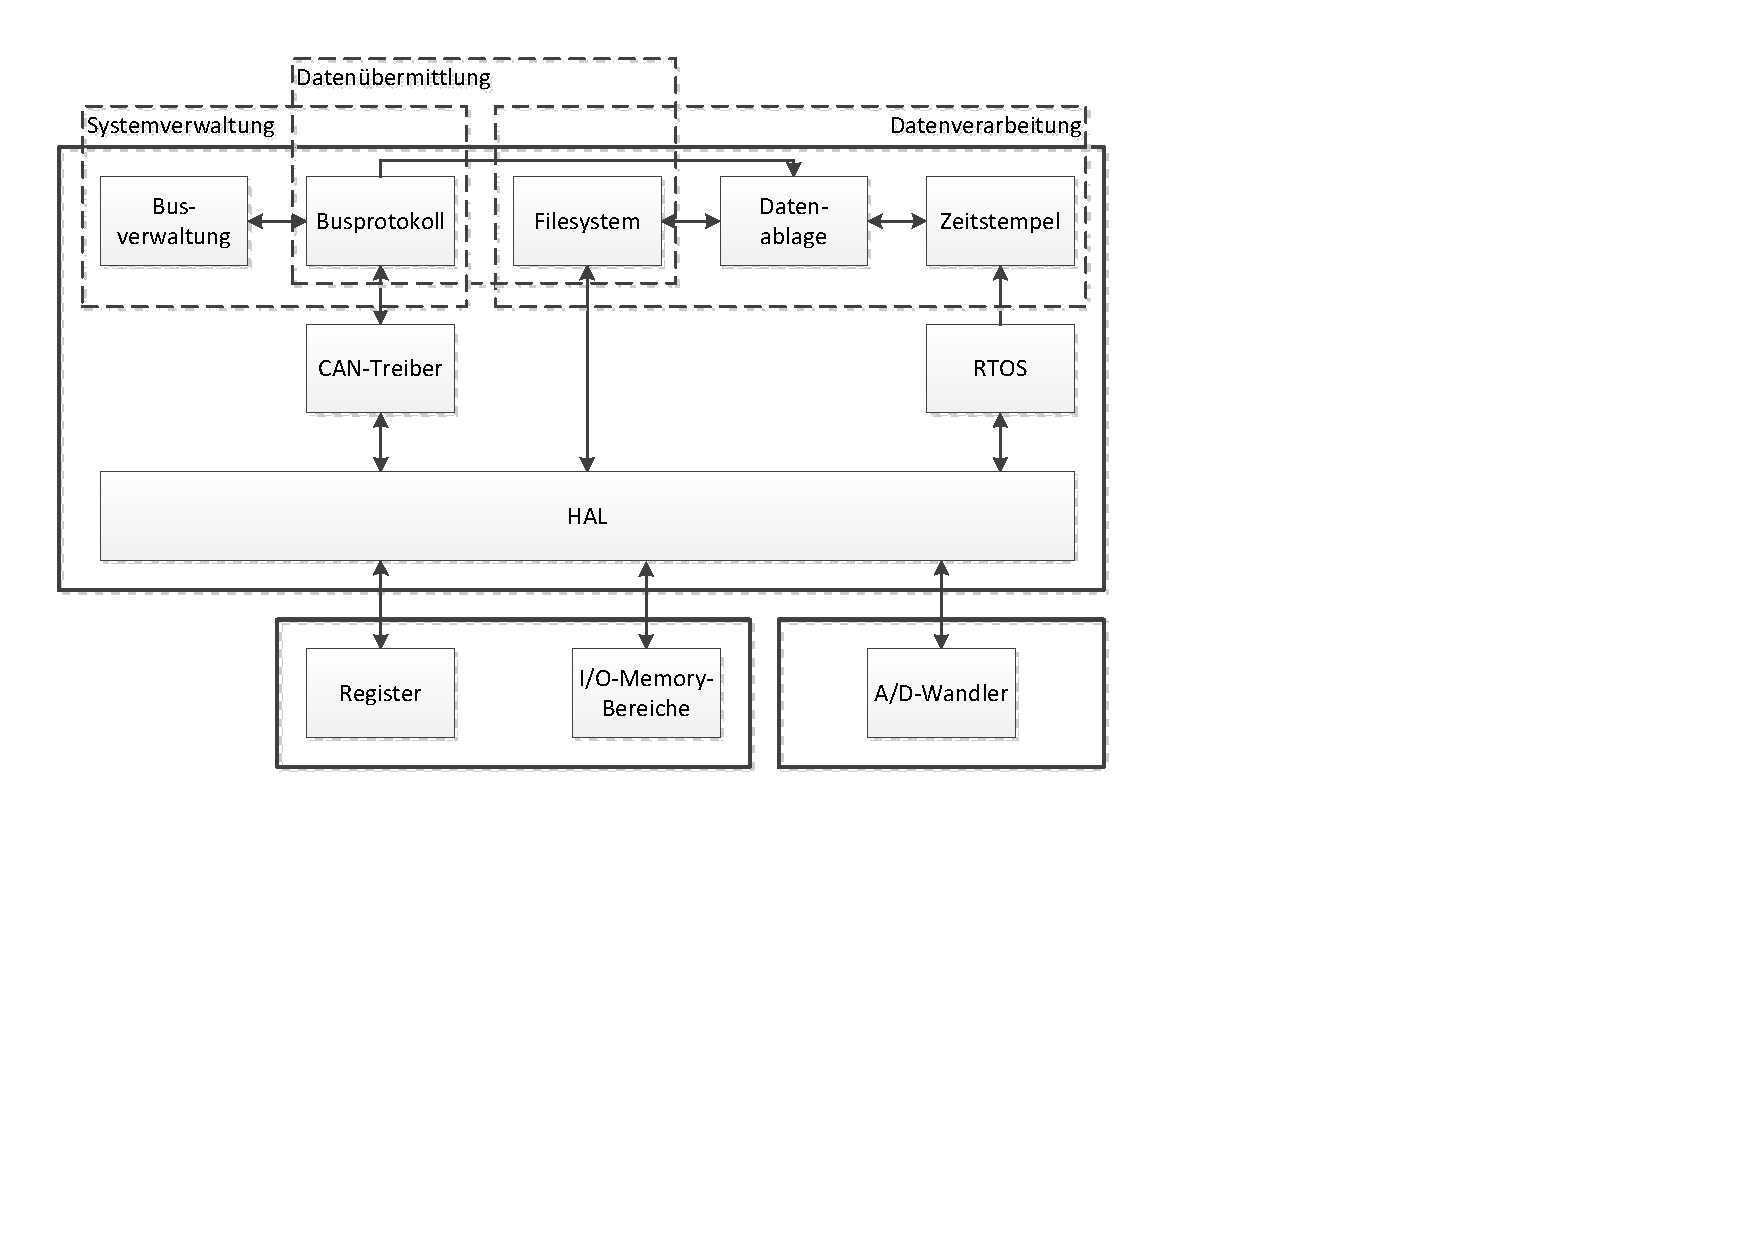
\includegraphics[width=0.8\textwidth]{images/visio/Softwarestack_Logger.pdf}
	\caption{Softwarestack des Datenloggers.}
	\label{fig.sw_logger}
\end{figure}

\begin{figure}[H]
	\centering
		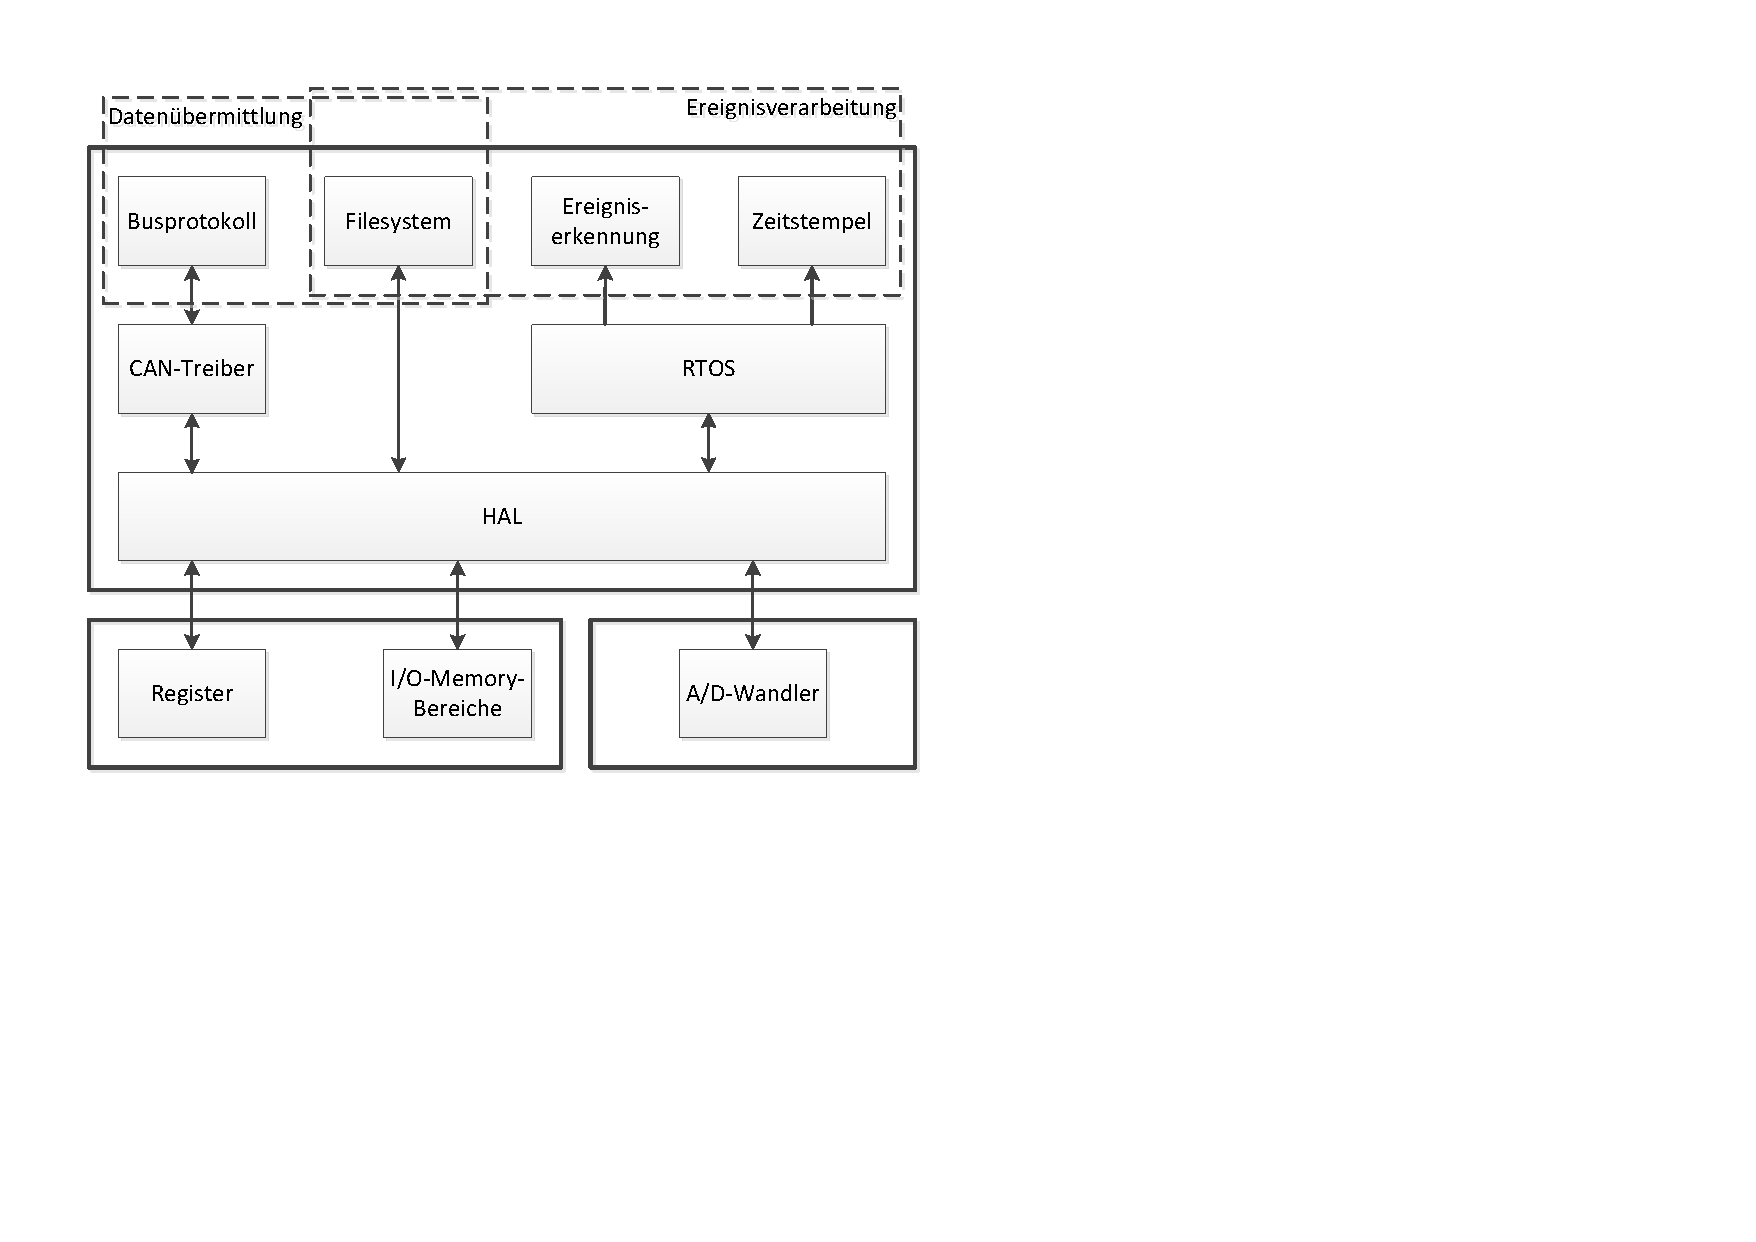
\includegraphics[width=0.8\textwidth]{images/visio/Softwarestack_Sensor.pdf}
	\caption{Softwarestack der Sensoreinheit.}
	\label{fig.sw_sensor}
\end{figure}



\subsection{Messdatenerfassung}\label{subsec.sw_messen}
Der NXP LPC4088 Microprozessor verfügt über einen 12-bit A/D-Wandler, der über einen Multiplexer auf acht Pins messen kann. Auf dem verwendeten Quickstart-Board stehen 6 Pins für A/D-Wandlung zur Verfügung. Für die geplante Anwendung reicht ein A/D-Eingang, da der Beschelunigungs-Sensor die Beschleunigung nur auf einer Achse misst. Der A/D-Wandler des NXP LPC4088 wird mit einer Samplingrate von 10 kHz betrieben. Falls höhere Samplingraten nötig sind, kann der A/D-Wandler mit bis zu 400 kHz betrieben werden.



\subsection{Ereigniserkennung}\label{subsec.sw_ereignis}
Vom WSL wurde die Ereigniserkennung bisher mittels Hilbert-Transformation gelöst. Die Hilbert-Transformation liefert die umhüllende Kurve des gemessenen Signals. Überschreitet die Umhüllende den Threshold, markiert dies den Start eines neuen Ereignisses. Fällt die Umhüllende unter den Threshold, ist das Ereignis beendet. Um den Rechenaufwand der Hilbert-Transformation zu umgehen, lösen wir die Ereigniserkennung einfacher.

\begin{figure}[H]
	\centering
		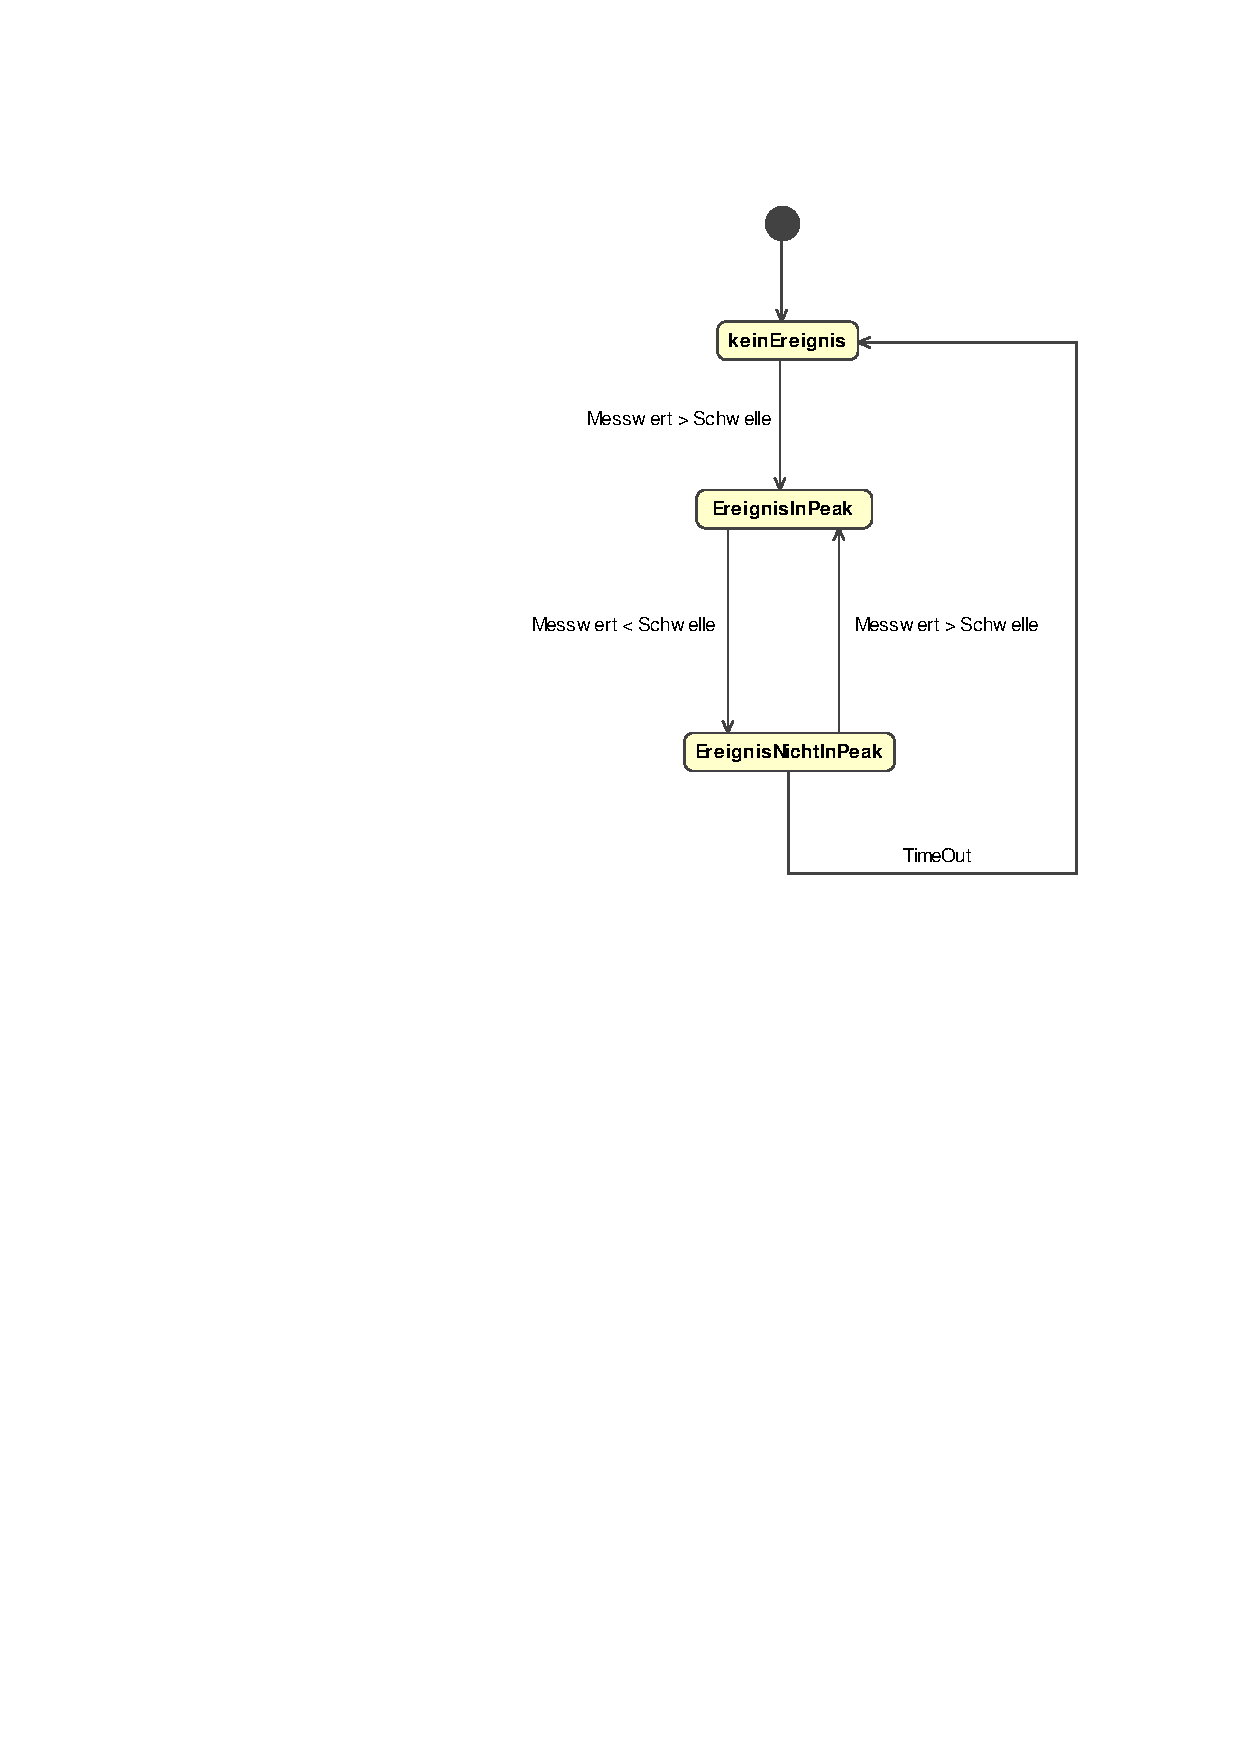
\includegraphics[width=0.8\textwidth]{images/magicdraw/Ereigniserkennung.pdf}
	\caption{Zustandsmaschine der Ereigniserkennung.}
	\label{fig.fsm_impact_detection}
\end{figure}

\todo{Ereigniserkennung beschreiben}

\subsection{Timestamp}\label{subsec.sw_timestamp}

\subsection{Verwaltung der Messstation}\label{subsec.sw_busverwaltung}
\todo{Busverwaltung beschreiben}

\begin{figure}[H]
	\centering
		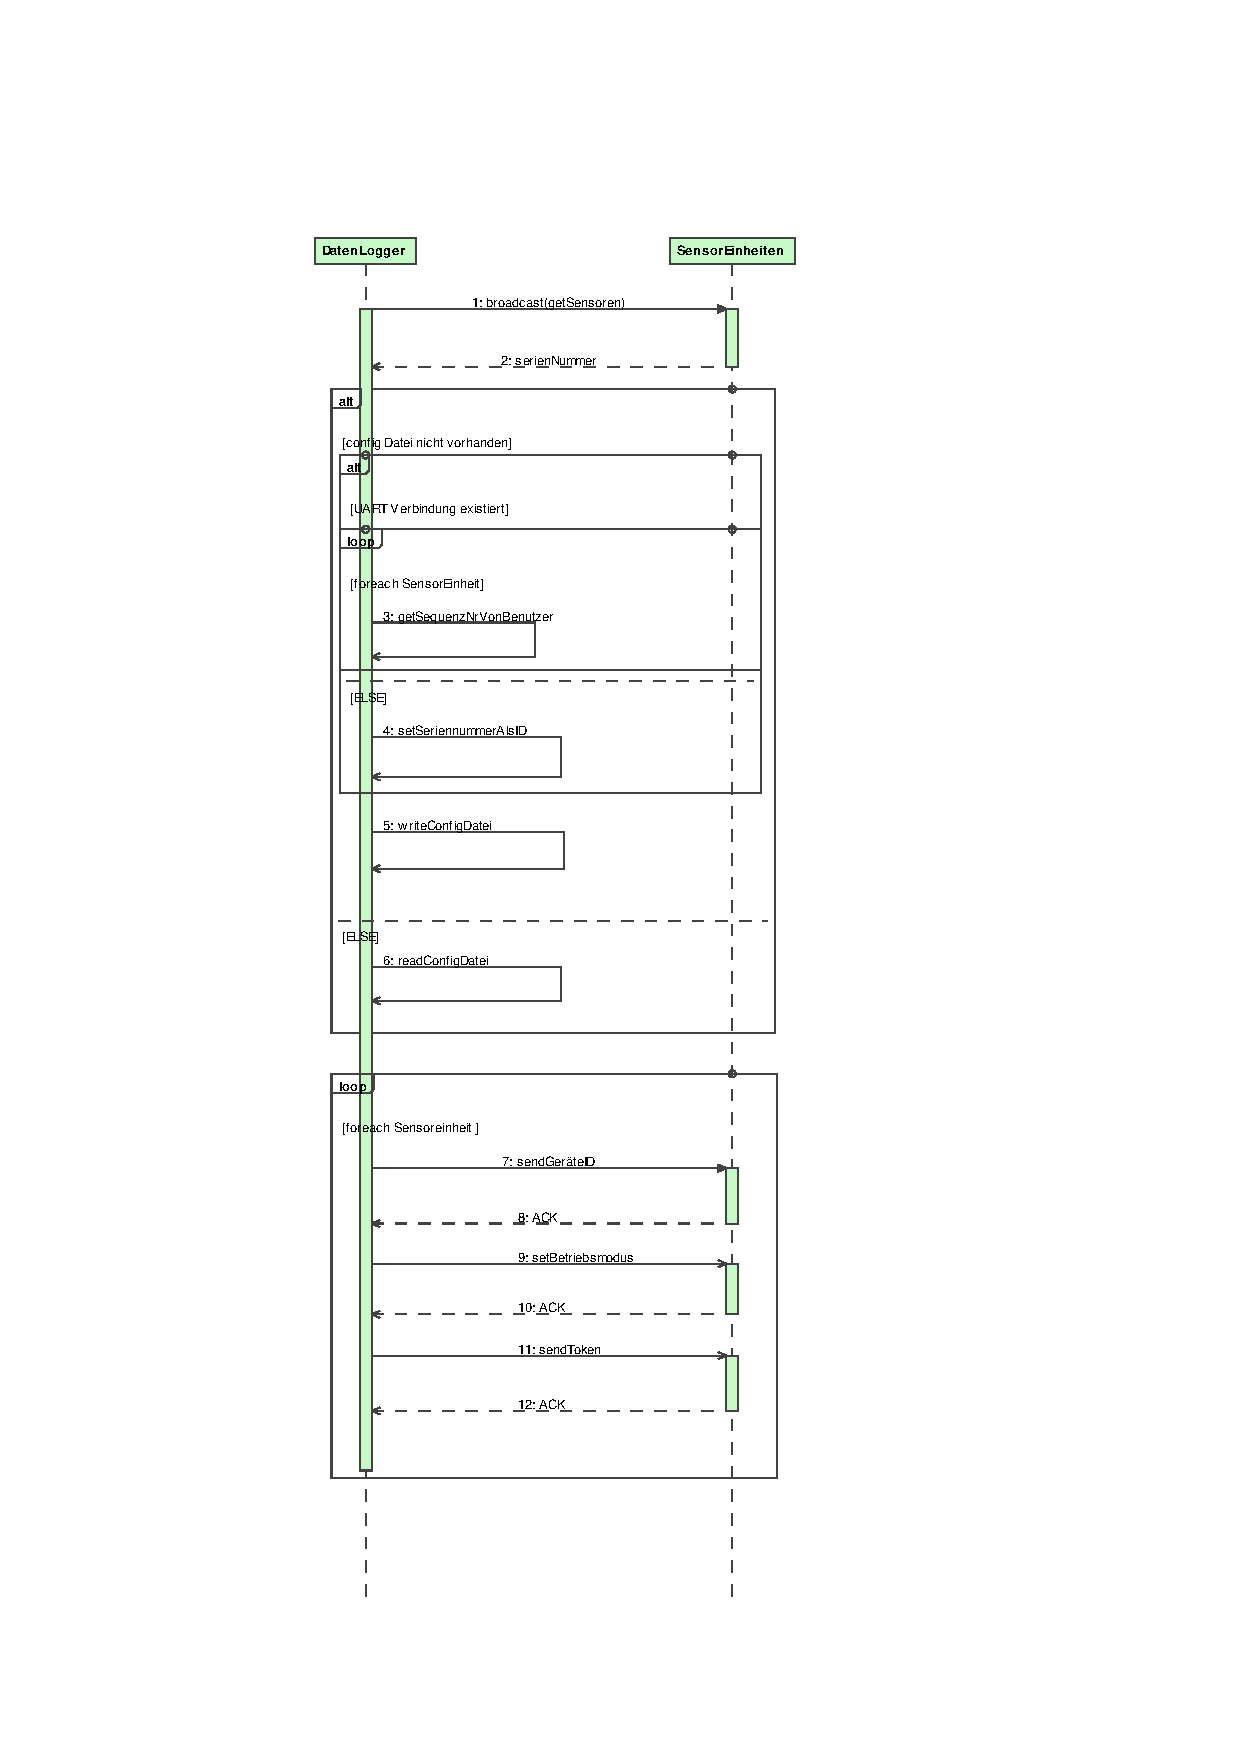
\includegraphics[height=0.9\textheight]{images/magicdraw/StartUpSequenz.pdf}
	\caption{Sequenzdiagramm des Startupvorgangs der Messstation.}
	\label{fig.seq_startup}
\end{figure}

\todo{Figur \ref{fig.seq_startup} aufteilen auf zwei Seiten. (PDF-crop)}

\subsection{Busprotokoll}\label{subsec.sw_busprotokoll}
\todo{Busprotokoll austüfteln. Darstellung siehe HW-Konzept Rioxo}

\subsection{Filesystem}\label{subsec.sw_filesystem}
\todo{Texten}

\subsection{UART-Kommandozeile}\label{subsec.sw_uart}
\todo{Texten}

\section{Funktionalität}\label{sec.sw_funktionalitaet}
\todo{Texten}

\section{Konfiguration}\label{sec.sw_konfiguration}
\todo{Texten}